\section{Aplicação Web}
\label{Sec:5-aplicativo-web}

Vários casos de uso especificados anteriormente possuem uma certa interdependência entre eles, por exemplo, o caso de uso Criar Meta necessita que o caso de uso Criar Equipamento esteja previamente desenvolvido. Para isso, adotou-se a seguinte ordem de implementação:

\begin{enumerate}
	\item{Fazer cadastro}
	\item{Fazer login}
	\item{Fazer logout}
	\item{Recuperar senha}
	\item{Criar equipamento}
	\item{Editar equipamento}
	\item{Remover equipamento}
	\item{Criar meta}
	\item{Editar meta}
	\item{Remover meta}
	\item{Atualizar taxas da AES}
	\item{Detectar sensores}
	\item{Editar sensor}
	\item{Remover sensor}
	\item{Configurar sistema}
	\item{Criar consumo}
	\item{Importar consumo}
	\item{Exportar consumo}
	\item{Visualizar consumo}
\end{enumerate}

\subsection{Models e Controllers}

Antes de implementar os casos de uso, as classes iniciais foram adaptadas para os Models do Django e a organização das classes no framework está representada na figura \ref{fig:diagrama-models}. Essas classes são responsáveis por acessar, criar, alterar ou remover dados dos equipamentos, sensores, taxas da AES, metas e usuários do banco de dados. Nos diagramas de classes simplificados a seguir foram representadas apenas as classes criadas para o projeto e as classes às quais estão diretamente relacionadas, ou seja, as demais classes do Django estão omitidas. A diferença observada em relação ao primeiro diagrama de classes (figura \ref{fig:diagrama-classes}) foi o fato de haver uma classe pré-existente User. A opção mais adequada para esse caso é criar um Model diferente (chamada Profile nesse caso) que tenha uma Foreign Key para um User. A partir de então, um usuário pode possuir um atributo adicional - income\_type - bastando criar um objeto da classe Profile e colocar uma Foreign Key para User. Essa é a opção mais adequada, uma vez que não é necessário criar uma nova classe de usuário, reescrevendo todos os atributos e métodos que o Django já oferece.

\begin{figure}
\centering
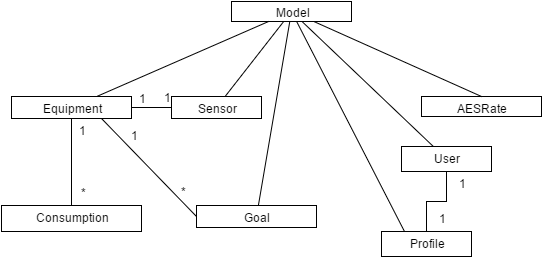
\includegraphics[width=14cm,keepaspectratio]{figuras/diagrama_models.png}
\caption{\label{fig:diagrama-models} Diagrama de Classes - Models}
\end{figure}

No projeto em questão são utilizados Controllers Principais (figura \ref{fig:diagrama-cont-principal}):
\begin{description}
	\item[IndexView:] Exibe página principal sem usuário logado.
	\item[HomeView:] Exibe página principal do usuário logado.
	\item[LoginView:] Exibe formulário para login e realiza autenticação.
	\item[LogoutView:] Encerra a sessão do usuário.
\end{description} 

\begin{figure}
\centering
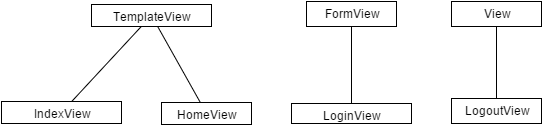
\includegraphics[width=14cm,keepaspectratio]{figuras/diagrama_cont_principal.png}
\caption{\label{fig:diagrama-cont-principal} Diagrama de Classes - Controllers Principais}
\end{figure}

Os Controllers que lidam com os equipamentos estão representados na figura \ref{fig:diagrama-cont-equipment}. E os Controllers são:
\begin{description}
	\item[IndexView:] Exibe página de listagem dos equipamentos.
	\item[CreateView:] Exibe página com formulário para criação de um equipamento, cria um equipamento, realiza redirecionamento após a criação.
	\item[UpdateView:] Exibe página com formulário para edição de um equipamento, edita um equipamento, realiza redirecionamento após a edição.
	\item[DeleteView:] Remove um equipamento.
\end{description} 

\begin{figure}
\centering
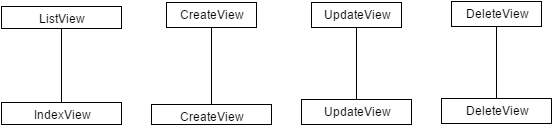
\includegraphics[width=14cm,keepaspectratio]{figuras/diagrama_cont_equipment.png}
\caption{\label{fig:diagrama-cont-equipment} Diagrama de Classes - Controllers de Equipamentos}
\end{figure}

Os Controllers que lidam com os sensores estão representados na figura \ref{fig:diagrama-cont-sensor}. E os Controllers são:
\begin{description}
	\item[IndexView:] Exibe página de listagem dos sensores.
	\item[UpdateView:] Exibe página com formulário para edição de um sensor, edita um sensor, realiza redirecionamento após a edição.
	\item[DeleteView:] Remove um sensor.
\end{description} 

\begin{figure}
\centering
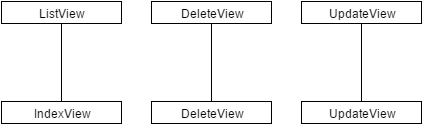
\includegraphics[width=10cm,keepaspectratio]{figuras/diagrama_cont_sensor.png}
\caption{\label{fig:diagrama-cont-sensor} Diagrama de Classes - Controllers de Sensores}
\end{figure}

Os Controllers que lidam com as taxas da AES estão representados na figura \ref{fig:diagrama-cont-aesrate}. E os Controllers são:
\begin{description}
	\item[IndexView:] Exibe página de listagem das taxas AES.
\end{description} 

\begin{figure}
\centering
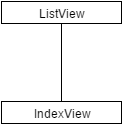
\includegraphics[width=3cm,keepaspectratio]{figuras/diagrama_cont_aesrate.png}
\caption{\label{fig:diagrama-cont-aesrate} Diagrama de Classes - Controllers de Taxas da AES}
\end{figure}

Os Controllers que lidam com as configurações do sistema (e do usuário) estão representados na figura \ref{fig:diagrama-cont-configuration}. E os Controllers são:
\begin{description}
	\item[ConfigView:] Exibe página com formulário para configuração do sistema, configura o sistema.
	\item[UserCreateView:] Exibe página com formulário para registro de um usuário, registra um usuário e realiza redirecionamento após registro.
	\item[UserUpdateView:] Exibe página com formulário para alteração dos dados de um usuário, altera os dados do usuário e realiza redirecionamento após alteração dos dados.
	\item[PasswordUpdateView:] Exibe página com formulário para edição de senha do usuário, edita a senha do usuário e redireciona após a alteração da senha.
	\item[PasswordRecoverView:] Exibe página com formulário para recuperação de senha do usuário, manda e-mail de recuperação de senha.
	\item[PasswordRecoverDoneView:] Redireciona depois do envio de e-mail para recuperação de senha.
	\item[PasswordResetView:] Exibe página com formulário para reconfigurar a senha do usuário, reconfigura a senha do usuário.
	\item[PasswordResetDoneView:] Redireciona depois da reconfiguração de senha do usuário.
\end{description} 

\begin{figure}
\centering
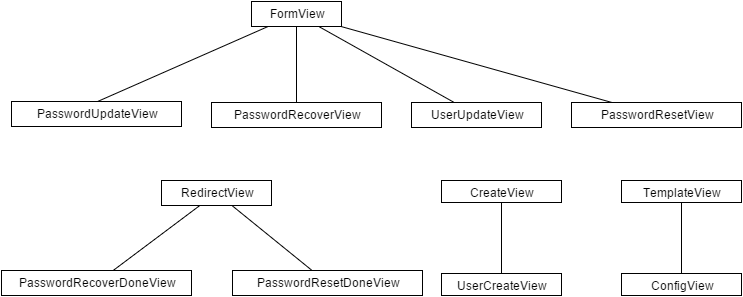
\includegraphics[width=16cm,keepaspectratio]{figuras/diagrama_cont_configuration.png}
\caption{\label{fig:diagrama-cont-configuration} Diagrama de Classes - Controllers de Configuração}
\end{figure}

Os Controllers que lidam com as metas estão representados na figura \ref{fig:diagrama-cont-goal}. E os Controllers são:
\begin{description}
	\item[IndexView:] Exibir página de listagem das metas.
	\item[CreateView:] Exibir página com formulário para criação de uma meta, cria uma meta, realiza redirecionamento após criar a meta.
	\item[UpdateView:] Exibir página com formulário para edição de uma meta, edita a meta, realiza redirecionamento após editar a meta.
	\item[DeleteView:] Remove uma meta.
\end{description} 

\begin{figure}
\centering
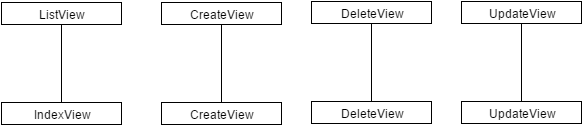
\includegraphics[width=14cm,keepaspectratio]{figuras/diagrama_cont_goal.png}
\caption{\label{fig:diagrama-cont-goal} Diagrama de Classes - Controllers de Metas}
\end{figure}

Os Controllers que lidam com os consumos estão representados na figura \ref{fig:diagrama-cont-consumption}. E os Controllers são:
\begin{description}
	\item[GraphicView:] Exibe o gráfico de consumo
\end{description} 

\begin{figure}
\centering
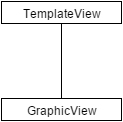
\includegraphics[width=3cm,keepaspectratio]{figuras/diagrama_cont_consumption.png}
\caption{\label{fig:diagrama-cont-consumption} Diagrama de Classes - Controllers de Consumos}
\end{figure}

No mesmo arquivo com os Controllers dos consumos estão localizados os métodos de criação do consumo (a ser chamado quando o Módulo Coordenador enviar uma requisição para a aplicação), importar consumos por arquivo CSV, exportar consumos por arquivo CSV e processar os dados para renderizar através do GraphicView.